\documentclass[12pt,a4paper]{report}
\usepackage{graphicx}
\usepackage{amsmath}
\usepackage{amssymb}
\usepackage{amsthm}
\usepackage{url}
\usepackage{hyperref}
\usepackage{setspace}
\usepackage{geometry}
\usepackage{background}
\usepackage{titlesec}
\usepackage{tabularx}
\usepackage{array}
\usetikzlibrary{calc}
\usepackage{blindtext}
\usepackage{etoolbox}
\usepackage{datetime}
\usepackage{lscape}
\usepackage{longtable}
\usepackage{float}
\usepackage{lipsum} % For generating dummy text
\usepackage{algorithm}
\usepackage{algorithmic}
%\usepackage[linesnumbered,ruled,vlined]{algorithm2e}
\usepackage{listings}
\usepackage{xcolor}
\usepackage{adjustbox}
\usepackage{rotating}
%\renewcommand{\qedsymbol}{}
% \usepackage{showframe}
%\usepackage{bera}
%\usepackage{mathptmx}  % Set Times New Roman as the font
\definecolor{codegray}{rgb}{0.5,0.5,0.5}
\definecolor{codegreen}{rgb}{0,0.6,0}
\definecolor{codeblue}{rgb}{0,0,0.8}
\definecolor{backcolor}{rgb}{0.95,0.95,0.92}

% Configure hyperref to make links blue
\hypersetup{
    colorlinks=true, % Use colored text instead of boxes
    citecolor=blue,  % Citations (e.g., [2]) in blue
    linkcolor=blue,  % Internal references (e.g., sections) in blue
    urlcolor=blue    % URLs in blue
}

\lstdefinestyle{mystyle}{
    backgroundcolor=\color{backcolor},   
    commentstyle=\color{codegreen},
    keywordstyle=\color{codeblue},
    numberstyle=\tiny\color{codegray},
    stringstyle=\color{codegreen},
    basicstyle=\ttfamily\footnotesize,
    breakatwhitespace=false,         
    breaklines=true,                 
    captionpos=b,                    
    keepspaces=true,                 
    numbers=left,                    
    numbersep=5pt,                  
    showspaces=false,                
    showstringspaces=false,
    showtabs=false,                  
    tabsize=2
}

\lstset{style=mystyle}

\renewcommand{\algorithmicrequire}{\textbf{Input:}}
\renewcommand{\algorithmicensure}{\textbf{Output:}}
\renewcommand{\algorithmiccomment}[1]{\hfill{\small\textit{#1}}}


\geometry{
 a4paper,
 total={170mm,257mm},
 left=20mm,
 top=20mm,
}

\backgroundsetup{angle=0, scale=1, vshift=-5ex,
  contents={\tikz[overlay, remember picture]
    \draw [rounded corners=7pt, line width=1.8pt,
           color=black, fill=white!50, double=black!120]
           ($(current page.north west)+(0.4cm,-0.4cm)$)
           rectangle ($(current page.south east)+(-0.4,0.4)$);}}

% \renewcommand{\cftchapaftersnum}{.}
% \renewcommand{\cftchappresnum}{\Roman{chapter}.~}

\titleformat{\chapter}[display]
  {\normalfont\bfseries} % overall formatting
  {\makebox[\textwidth][l]{\fontsize{36}{42}\selectfont\chaptername\ \thechapter}} % prints "Chapter 1" at top-right
  {0pt} % separation between label and title
  {\centering\fontsize{28}{34}\selectfont} % centers and sizes the chapter title
  []

\titlespacing*{\chapter}{0pt}{0pt}{14pt}
% ----------------------------------------------------------------------

\titleformat{\section}
  {\normalfont\fontsize{12}{14}\bfseries}{\thesection}{1em}{}
\titlespacing*{\section}{0pt}{*2}{*1.5}

\titleformat{\subsection}
  {\normalfont\fontsize{12}{14}\bfseries\itshape}{\thesubsection}{1em}{}
\titlespacing*{\subsection}{0pt}{*1.5}{*1}

\titleformat{\subsubsection}
  {\normalfont\fontsize{12}{14}\bfseries\itshape}{\thesubsubsection}{1em}{}
\titlespacing*{\subsubsection}{0pt}{*1}{*0.5}

\newdateformat{mydateformat}{\twodigit{\THEDAY}-\twodigit{\THEMONTH}-\THEYEAR}
% \date{\mydateformat\today}

\usepackage{fancyhdr} % Add this package
\fancypagestyle{plain}{% Define the plain page style for non-chapter pages
  \fancyhf{}
  \renewcommand{\headrulewidth}{0pt}
  \renewcommand{\footrulewidth}{0pt}
}

\fancypagestyle{chapterstyle}{% Define the chapterstyle for chapter pages
  \fancyhf{}
  \fancyhead[L]{\leftmark} % Left header contains the chapter title
  \fancyhead[R]{\thepage} % Right header contains the page number
  \fancyfoot[C]{\small B.M.S College of Engineering, Bangalore} % Center footer contains the course name
  \renewcommand{\headrulewidth}{1.5pt} % Line thickness for header
  \renewcommand{\footrulewidth}{1.0pt} % Line thickness for footer
}

% Define theorem environments
\newtheorem{theorem}{Theorem}
\newtheorem{lemma}[theorem]{Lemma} % Lemmas are numbered as theorems
\newtheorem{corollary}[theorem]{Corollary}

\theoremstyle{definition}
\newtheorem{definition}{Definition}

\theoremstyle{remark}
\newtheorem{remark}{Remark}

% Keep report tables inside the text block while allowing longtable page breaks.
\newcolumntype{L}[1]{>{\raggedright\arraybackslash}p{#1}}
\newcolumntype{C}[1]{>{\centering\arraybackslash}p{#1}}
\newcolumntype{R}[1]{>{\raggedleft\arraybackslash}p{#1}}
\setlength{\tabcolsep}{2pt}
\AtBeginEnvironment{longtable}{%
  \footnotesize
  \renewcommand{\baselinestretch}{1.0}\selectfont
  \setlength{\tabcolsep}{2pt}%
  \renewcommand{\arraystretch}{0.95}%
  \setlength{\LTleft}{0pt}%
  \setlength{\LTright}{0pt}%
}

\begin{document}
\linespread{1.39}\selectfont
\pagestyle{plain} % Use plain style for the title page

\begin{titlepage}
    \begin{center}
        \textsc{\Large \textbf{\textcolor{blue}{B.M.S. COLLEGE OF ENGINEERING}}}\\[0.2cm]
        \textsc{\large \textbf{(Autonomous College under VTU)}}\\[0.2cm]
        \textsc{\large \textbf{Bull Temple Road, Basavangudi, Bangalore - 560019}}\\[0.5cm]
        
        \includegraphics[scale=0.75]{logo.png}\\[0.18cm]
        \textit{Report on}\\[0.18cm]
        \textsc{\textbf{\textcolor{black}{A SAM-Based Synthetic Data Pipeline for UAV-Style Crop Disease Detection}}}\\[0.2cm]
        \textit{submitted as the Project Management Capstone Report for the course}\\[0.18cm]
        \textbf{Entrepreneurship \& Project Management (23DC7PCEPM)}\\[0.15cm]
        \textit{in fulfillment of the requirements for the award of degree}\\[0.2cm]
        
        \textbf{BACHELOR OF ENGINEERING}\\[0.15cm]
        \textit{in}\\[0.2cm]
        \textbf{Computer Science \& Engineering (Data Science)}\\[0.2cm]
        
        \textit{ by}\\[0.2cm]
         \textbf{{Hemanth R (1BM23CD021)}}\\[0.2cm]
        \textbf{{Vedantha Vinay Vernekar (1BM23CD069)}}\\[0.2cm]
          \textbf{{Shakthi Jashwanth CH (1BM23CD072)}}\\[0.2cm]

        \textbf{Under the Guidance of}\\[0.25cm]
        \textbf{Prof. Lavanya Naik}\\[0.15cm]
        Assistant Professor\\[0.55cm]
        \textbf{Department of CSE (Data Science)}, \\
        \textbf{B.M.S. College of Engineering}\\[0.25cm]

        \textbf{AY 2026-2027}
    \end{center}
\end{titlepage}

\pagenumbering{arabic}
\renewcommand{\contentsname}{Contents}
\tableofcontents
\newpage

\begin{center}
{\LARGE\bfseries\color{navy} PROJECT MANAGEMENT}\par
{\Large\bfseries\color{navy} Project Work -- Phase II}\par
{\large\itshape AgroEye: A SAM-Based Synthetic Data Pipeline for UAV-Style Crop Disease Detection}
\end{center}

\section{Executive Summary}
AgroEye is an annotation-free synthetic-data pipeline for UAV-style crop disease detection. It extracts real diseased leaves from PlantVillage images with Segment Anything (SAM), composes them onto real aerial ground tiles with domain randomisation, produces automatic YOLO labels from the pasted masks, and evaluates CNN and Transformer detectors on synthetic and real UAV imagery.

The completed pipeline produced 18,163 SAM cutouts across 13 classes, used 6,652 selected cutouts, generated 1,200 synthetic composites and produced 57,771 boxes without manual annotation. YOLOv11m achieved 0.907 mAP@50, 0.733 mAP@50--95 and 67.7 FPS on the held-out synthetic test split. In the real UAV transfer study, synthetic pretraining improved mean patch-level AUC from 0.59 to 0.68 with full real data across three seeds, although the gain was plot-dependent.

The project also delivered an in-browser ONNX demo. The real-UAV study was partial because the available public dataset supplied patch labels rather than bounding boxes. The main limitations are no zero-shot or low-data gain, no completed factor ablation, shared assets and one synthetic-training seed.

\subsection{Project Facts and Baseline}
\begin{longtable}{|L{.34\linewidth}|L{.54\linewidth}|}
\hline
\hrow\hc{Measure}&\hc{Verified value}\\
\hline\endhead
PlantVillage source & 18,163 images, 13 classes\\\hline
Selected cutouts & 6,652 from 18,163; automatic prompts 12,881 and centre prompts 5,281\\\hline
SAM extraction & 0.12 images/s, approximately 41 hours\\\hline
Aerial sources and tiles & 65 source images, 176 native-resolution 640 px tiles\\\hline
Background categories & 47 soil, 25 farm and 104 grass tiles\\\hline
Synthetic dataset & 1,200 composites, 57,771 boxes, 48.1 mean leaves/image\\\hline
Dataset split & Seed 42; 960/120/120 images and 46,561/5,285/5,925 boxes\\\hline
Class balance & 9,488--9,770 boxes per class; 152--1,909 distinct cutouts per class\\\hline
Hardware & RTX A5000 24 GB, Xeon W-2295, 128 GB RAM\\\hline
\end{longtable}

\section{Project Foundation}
\subsection{Project Attributes}
\begin{longtable}{|L{.27\linewidth}|L{.65\linewidth}|}
\hline
\hrow\hc{Attribute}&\hc{AgroEye evidence}\\
\hline\endhead
Clear objective & Build an annotation-free UAV-style disease detector and test transfer to real UAV imagery.\\\hline
Interdependent activities & SAM cutouts feed the compositor; the compositor creates labels; labels feed detector training; evaluation depends on leakage-safe splits.\\\hline
Various resources & Three students, two faculty guides, one RTX A5000 workstation, PlantVillage, aerial tiles, public real-UAV data and open-source software.\\\hline
Specific time frame & Review 2 project window: 06 Jul--13 Nov 2026; 19 planned weeks.\\\hline
Unique effort & Combines real photographed lesions, SAM mask selection, seven-factor composition, rotated-alpha labels, two detectors and plot-level transfer evaluation.\\\hline
Customers and proxies & Smallholder farmers, agronomists, extension officers, drone service providers, evaluators and faculty guides.\\\hline
Uncertainty & Synthetic-to-real scale and camera differences were unknown; zero-shot AUC was 0.48 and full-data transfer reached 0.68.\\\hline
\end{longtable}

\subsection{Balancing Project Constraints}
\begin{longtable}{|L{.18\linewidth}|c|L{.28\linewidth}|L{.34\linewidth}|}
\hline
\hrow\hc{Constraint}&\hc{Priority}&\hc{Target or limit}&\hc{Project decision}\\
\hline\endhead
Quality & 1 & Reliable labels, leakage-free splits, mAP/AUC and speed reported together & Use parsed labels, held-out synthetic evaluation and leave-one-plot-out real evaluation.\\\hline
Schedule & 2 & Finish the review and paper in the fixed academic window & Run WP9 in parallel and track weekly milestones.\\\hline
Scope & 3 & Synthetic pipeline, two detectors, transfer study and demo & Exclude drone hardware, flight planning, cloud deployment and multispectral data.\\\hline
Customer satisfaction & 4 & Mentor and evaluator acceptance & Weekly reviews, documented limitations and reproducible figures.\\\hline
Resources & 5 & One GPU workstation and three students & Cache cutouts, tiles and experiment results; run GPU jobs serially.\\\hline
Budget & 6 & Notional student effort; no cash purchases & Track person-days, mentor hours and reserve use.\\\hline
Risk & 7 & Control scale gap, leakage, GPU failure and number drift & Use plot-level CV, audit scripts, cache recovery and a change log.\\\hline
\end{longtable}

\subsection{Stakeholder Engagement}
\begin{longtable}{|L{.27\linewidth}|L{.27\linewidth}|c|L{.27\linewidth}|}
\hline
\hrow\hc{Stakeholder}&\hc{Interest}&\hc{Influence}&\hc{Engagement}\\
\hline\endhead
Project team & Deliver a working pipeline, report and demo & H & Weekly coordination and shared repository.\\\hline
Faculty guides & Academic rigour, scope and review quality & H & Milestone reviews and approval of changes.\\\hline
Agronomists and extension officers & Field-wide, early crop-disease warning & M & Requirements and limitations mapped to field use.\\\hline
Smallholder farmers & Affordable early warning & M & Treated as intended beneficiaries, not deployment users.\\\hline
Drone service providers & Models without heavy manual labelling & M & Throughput and annotation cost reported.\\\hline
Evaluators and department & Meets Phase II and PM outcomes & H & Report, evidence tables and review presentation.\\\hline
Open-source community & Reproducible research & L & Pinned versions, scripts, seeds and documented caveats.\\\hline
\end{longtable}

\subsection{Project Charter}
\begin{longtable}{|L{.30\linewidth}|L{.62\linewidth}|}
\hline
\hrow\hc{Charter field}&\hc{AgroEye decision}\\
\hline\endhead
Purpose & Reduce the cost of creating labelled UAV-style crop-disease training data by composing real photographed lesions onto real aerial backgrounds.\\\hline
Project manager & Hemanth R; coordinates work, reviews evidence and escalates scope or schedule changes to the guides.\\\hline
Measurable objective & Deliver 1,200 synthetic scenes, automatic labels, two benchmarked detectors, real-UAV transfer evidence, a demo and a PM report by 13 Nov 2026.\\\hline
Acceptance criteria & 57,771 parsed boxes, valid split files, reproducible held-out metrics, documented real-UAV protocol, speed measurement and code audit.\\\hline
In scope & SAM extraction, background tiling, seven-factor compositor, YOLO labels, YOLOv11m, RT-DETR-L, real-UAV CV, ONNX demo, paper and report.\\\hline
Out of scope & Drone operation, flight planning, cloud service, multispectral sensing, field deployment and unverified ablation claims.\\\hline
Assumptions & Public datasets are available, the workstation remains usable, and the public real-UAV data can support plot-level validation.\\\hline
Constraints & One GPU, no in-house annotated flights, shared synthetic assets, limited review time and no automated unit-test suite.\\\hline
Approval & Guides review the baseline, changes, results and report before submission.\\\hline
\end{longtable}

\subsection{Life Cycle and Planning Process}
\begin{longtable}{|L{.20\linewidth}|L{.25\linewidth}|L{.45\linewidth}|}
\hline
\hrow\hc{Phase}&\hc{Dates}&\hc{Work performed}\\
\hline\endhead
Initiating & 06--10 Jul 2026 & Problem, stakeholders, objectives, constraints and acceptance measures defined.\\\hline
Planning & 06--17 Jul 2026 & WBS, owners, activity durations, budget, Gantt baseline and risk register prepared.\\\hline
Performing & 20 Jul--30 Oct 2026 & Assets, SAM extraction, composition, labels, detector training, evaluation and transfer CV completed.\\\hline
Closing & 31 Oct--13 Nov 2026 & Audit, report, paper revisions, demo readiness and final review evidence.\\\hline
\end{longtable}

\subsection{Introduction and Problem Statement}
Early and late blight reduce tomato and potato yields; UAVs image fields at centimetre resolution on demand. No large UAV-view dataset boxes every diseased leaf. One frame holds dozens of small targets, so labelling is slow. PlantVillage [1] shows single close-up leaves and its models degrade in the field [2]. Cut-and-paste [3] and domain randomisation [4] work elsewhere, while agricultural synthetic data uses generated targets [6, 7].

The scope is SAM extraction, a seven-factor compositor, automatic labels, two detectors and a real-UAV transfer test. Drone hardware, flight planning, cloud deployment and multispectral imaging are excluded.

\subsection{Two Imaging Regimes}
\begin{longtable}{|L{.25\linewidth}|L{.29\linewidth}|L{.29\linewidth}|}
\hline
\hrow\hc{Property}&\hc{PlantVillage}&\hc{UAV nadir}\\
\hline\endhead
Geometry & One centred leaf & Top-down, many plants\\\hline
Background & Uniform & Soil, weeds, crop rows\\\hline
Lighting & Controlled, diffuse & Direct sun, shadow\\\hline
Scale & Leaf fills the frame & 29--74 px in 640 px\\\hline
Occlusion & None & Overlapping canopy\\\hline
\end{longtable}
Naive pasting gives a ``sticker effect'': hard edges, no contact shadow, wrong scale and wrong colours.

\subsection{Objectives}
\begin{longtable}{|L{.08\linewidth}|L{.39\linewidth}|L{.12\linewidth}|L{.30\linewidth}|}
\hline
\hrow\hc{ID}&\hc{Objective}&\hc{Status}&\hc{Evidence}\\
\hline\endhead
O1 & Extract background-free leaf cutouts without manual masks & Completed & 18,163 SAM cutouts, 13 classes; 6,652 used\\\hline
O2 & Compose UAV-style scenes with domain randomisation and automatic YOLO labels & Completed & 1,200 composites, 57,771 boxes, 0 manual labels\\\hline
O3 & Train and benchmark CNN and Transformer detectors & Completed & YOLOv11m 0.907 versus RT-DETR-L 0.761 mAP@50\\\hline
O4 & Fine-tune on real drone imagery (reality loop) & Partial & Public UAV data used; AUC 0.59 to 0.68, gain on 2 of 4 plots\\\hline
O5 & Demonstrate the trained detector & Completed & In-browser ONNX demo (PWA)\\\hline
\end{longtable}
O4 changed scope because no annotated in-house flights were available; the public A. solani UAV dataset [8] was used instead. It contains patch labels, not boxes.

\section{Project Planning}
\subsection{Project Objective}
Deliver by 13 Nov 2026 a reproducible synthetic-data pipeline that generates 1,200 UAV-style scenes and 57,771 automatic boxes, benchmarks YOLOv11m against RT-DETR-L, evaluates transfer on plot-level real-UAV folds, and provides an offline-capable browser demo. Success means the data, split, metrics, limitations and code can be independently rechecked.

\subsection{Project Scope Document}
\begin{longtable}{|L{.28\linewidth}|L{.62\linewidth}|}
\hline
\hrow\hc{Scope section}&\hc{AgroEye definition}\\
\hline\endhead
Customer requirement & Reduce manual UAV disease-box annotation while preserving realistic lesions, scale variation and field backgrounds.\\\hline
Statement of work & Collect PlantVillage and aerial assets; extract SAM masks; tile backgrounds; compose scenes; generate labels; train, test and compare detectors; run real-UAV CV; document.\\\hline
Deliverables & Cutout library, tiled background library, 1,200-composite dataset, 57,771 labels, YOLOv11m and RT-DETR-L checkpoints, evaluation tables, ONNX demo, paper and PM report.\\\hline
Acceptance measures & Parsed labels, no split or plot leakage, synthetic mAP and speed figures reproduced, real AUC reported with fold and seed details, limitations stated.\\\hline
Out of scope & Own drone flights, field deployment, cloud inference, multispectral sensing, manual box annotation and unverified ablation results.\\\hline
\end{longtable}

\subsection{Plan for Quality}
\begin{longtable}{|L{.23\linewidth}|L{.27\linewidth}|L{.35\linewidth}|}
\hline
\hrow\hc{Quality measure}&\hc{Target}&\hc{How checked}\\
\hline\endhead
Cutout validity & 18,163 non-empty single-component outputs & File audit after SAM extraction; failed write reprocessed.\\\hline
Label integrity & 57,771 parsed boxes; 0 invalid & Parse every YOLO file rather than count newlines.\\\hline
Split integrity & No image in two synthetic splits & Compare image identifiers after seed-42 split.\\\hline
Leakage control & No plot in two real-CV partitions & Leave-one-plot-out fold audit.\\\hline
Discrimination & Report mAP@50, mAP@50--95, AUC and AP & Re-evaluate stored checkpoints and cached fold results.\\\hline
Sensitivity to threshold & F1 threshold chosen on validation data & Do not use a fixed test-derived threshold.\\\hline
Reproducibility & Fixed seeds and pinned versions & Compare training arguments, checkpoints and stored results.\\\hline
\end{longtable}

\subsection{Responsibility Assignment Matrix}
\begin{longtable}{|L{.34\linewidth}|c|c|c|c|}
\hline
\hrow\hc{Work package}&\hc{Hemanth}&\hc{Shakthi}&\hc{Vedantha}&\hc{Guides}\\
\hline\endhead
WP1 Literature and problem definition & P & S & S & S\\\hline
WP2 Asset collection & S & S & P & S\\\hline
WP3 SAM leaf extraction & S & P & S & S\\\hline
WP4 Compositor and labelling & P & S & S & S\\\hline
WP5 Dataset packaging & S & P & S & S\\\hline
WP6 Detector training & S & S & P & S\\\hline
WP7 Evaluation and analysis & P & S & S & S\\\hline
WP8 Real-UAV transfer study & S & P & S & S\\\hline
WP9 Demo application & S & S & P & S\\\hline
WP10 Paper and report & P & S & S & P\\\hline
\end{longtable}

\subsection{Proposed Methodology}
Cut real diseased leaves out of lab photos with SAM, paste them onto real aerial ground tiles at drone scale with randomised nuisance factors, and compute every box from the pasted leaf's own mask. Manual box labelling is too slow and costly. GAN or diffusion targets [6, 7] create synthetic textures; AgroEye keeps real photographed lesions. Leaf-Only SAM [9] scores green leaves only; AgroEye also credits yellow--brown diseased tissue.

\subsection{SAM Mask Score}
\[
s(M)=0.20A+0.28C+0.30G+0.12\hat q+0.10\sigma-0.25B
\]
$A$ is area preference with a peak at 30\% of the image, $C$ is centrality, $G$ is HSV plant colour including green and yellow--brown, $\hat q$ and $\sigma$ are SAM predicted IoU and stability, and $B$ is border contact.

\subsection{Rotation-Aware YOLO Label}
\[
x_c=\frac{x_{\min}+w/2}{W},\qquad y_c=\frac{y_{\min}+h/2}{H},\qquad w'=\frac{w}{W},\qquad h'=\frac{h}{H}
\]
The extent of rotated alpha is greater than 20; $W=H=640$, and all values are clamped to $[0,1]$.

\subsection{Seven Compositor Factors}
\begin{longtable}{|c|L{.33\linewidth}|L{.45\linewidth}|}
\hline
\hrow\hc{No.}&\hc{Factor}&\hc{Applied range or rule}\\
\hline\endhead
1 & GSD scaling & Leaf width 4.5--11.5\% of 640 px (29--74 px)\\\hline
2 & Rotation & Uniform angle from 0 to 360 degrees\\\hline
3 & Alpha feathering & Gaussian radius 0.8 px\\\hline
4 & Drop shadow & Offset (2,3) px, blur 2 px, opacity 0.30\\\hline
5 & Canopy clustering & 2--5 plant centres; 80\% clustered leaves; $\sigma=40$--95 px; IoU guard 0.50\\\hline
6 & Photometric jitter & Leaf brightness 0.85--1.20, saturation 0.80--1.20; tile brightness 0.85--1.15\\\hline
7 & Sensor blur & Probability 0.25, radius 0.4--0.9 px\\\hline
\end{longtable}
The target canopy mix is 15--28 leaves with probability 0.2, 35--65 with probability 0.6, and 66--95 with probability 0.2. Placements above IoU 0.50 are skipped rather than retried, giving 48.1 realised leaves per image. The assumed camera scale is approximately 0.25 cm per pixel, not a calibrated camera model.

\subsection{Work Breakdown Structure}
\begin{longtable}{|c|L{.31\linewidth}|L{.28\linewidth}|L{.17\linewidth}|c|}
\hline
\hrow\hc{WP}&\hc{Work package}&\hc{Owner}&\hc{Planned (2026)}&\hc{Weeks}\\
\hline\endhead
1 & Literature, problem definition & Hemanth R & 06--24 Jul & 3\\\hline
2 & Asset collection & Vedantha V V & 27 Jul--07 Aug & 2\\\hline
3 & SAM leaf extraction & Shakthi Jashwanth CH & 10--28 Aug & 3\\\hline
4 & Compositor and labelling & Hemanth R & 31 Aug--11 Sep & 2\\\hline
5 & Dataset packaging & Shakthi Jashwanth CH & 14--18 Sep & 1\\\hline
6 & Detector training & Vedantha V V & 21--25 Sep & 1\\\hline
7 & Evaluation and analysis & Hemanth R & 28 Sep--09 Oct & 2\\\hline
8 & Real-UAV transfer study & Shakthi Jashwanth CH & 12--30 Oct & 3\\\hline
9 & Demo application & Vedantha V V & 28 Sep--09 Oct & 2\\\hline
10 & Paper and report & Hemanth R & 02--13 Nov & 2\\\hline
\end{longtable}
The critical path total is 06 Jul--13 Nov, 19 weeks. Weeks are Monday--Friday; W1 starts 06 Jul 2026. WP9 is off the critical path. For WP9, $ES_9=EF_6$ at the end of W12 (25 Sep), $LF_9=LS_{10}$ at the end of W17 (30 Oct), and slack is $17-(12+2)=3$ weeks.

\section{Developing the Schedule}
\subsection{Activity List, Resources and Durations}
\begin{longtable}{|c|L{.27\linewidth}|L{.13\linewidth}|L{.24\linewidth}|c|}
\hline
\hrow\hc{WP}&\hc{Activity}&\hc{Predecessor}&\hc{Resources and effort}&\hc{Weeks}\\
\hline\endhead
1 & Literature and problem definition & -- & Hemanth; 3 weeks & 3\\\hline
2 & Asset collection & 1 & Vedantha; 2 weeks & 2\\\hline
3 & SAM leaf extraction & 2 & Shakthi; 41 GPU hours & 3\\\hline
4 & Compositor and labelling & 3 & Hemanth; compositor iterations & 2\\\hline
5 & Dataset packaging & 4 & Shakthi; split and audit & 1\\\hline
6 & Detector training & 5 & Vedantha; two 40-epoch runs & 1\\\hline
7 & Evaluation and analysis & 6 & Hemanth; test and threshold metrics & 2\\\hline
8 & Real-UAV transfer study & 7 & Shakthi; four plot folds and seeds & 3\\\hline
9 & Demo application & 7 & Vedantha; ONNX and Web Worker & 2\\\hline
10 & Paper and report & 8, 9 & Hemanth; review and release & 2\\\hline
\end{longtable}

\subsection{Network Diagram and Schedule Calculations}
The critical path is WP1 $\rightarrow$ WP2 $\rightarrow$ WP3 $\rightarrow$ WP4 $\rightarrow$ WP5 $\rightarrow$ WP6 $\rightarrow$ WP7 $\rightarrow$ WP8 $\rightarrow$ WP10. It spans 19 weeks. WP9 is parallel to WP7 and WP8. Its earliest start is after WP6, its latest finish is before WP10, and its available slack is 3 weeks.

\begin{longtable}{|c|c|c|c|c|c|c|}
\hline
\hrow\hc{WP}&\hc{Duration}&\hc{ES}&\hc{EF}&\hc{LS}&\hc{LF}&\hc{Slack}\\
\hline\endhead
1 & 3 & 0 & 3 & 0 & 3 & 0\\\hline
2 & 2 & 3 & 5 & 3 & 5 & 0\\\hline
3 & 3 & 5 & 8 & 5 & 8 & 0\\\hline
4 & 2 & 8 & 10 & 8 & 10 & 0\\\hline
5 & 1 & 10 & 11 & 10 & 11 & 0\\\hline
6 & 1 & 11 & 12 & 11 & 12 & 0\\\hline
7 & 2 & 12 & 14 & 12 & 14 & 0\\\hline
8 & 3 & 14 & 17 & 14 & 17 & 0\\\hline
9 & 2 & 12 & 14 & 15 & 17 & 3\\\hline
10 & 2 & 17 & 19 & 17 & 19 & 0\\\hline
\end{longtable}
For WP9, total slack is $LS-ES=15-12=3$ weeks and free slack is $ES_{10}-EF_9=17-14=3$ weeks. A five-day delay on the critical path would move the planned finish by five days because all critical activities have zero slack.

\subsection{Project Control Process}
The team reviewed progress weekly. Each review recorded actual dates, effort, percent complete, dataset counts, mAP/AUC, risks and corrective action. A corrective action was triggered by a critical-path slip, a failed output audit, a GPU failure, a suspiciously high random-split score, or a metric that could not be reproduced from stored results. The baseline was fixed at project initiation and all scope changes were recorded.

\subsection{Schedule Variance and Change Control}
The synthetic dataset and detector training finished ahead of the planned dates. Repository and LFS tracking finished on 26 Oct rather than 09 Oct, but did not move the paper review because the report work was pulled forward. The GPU crash stopped four of sixteen multi-seed runs; serial execution and cache recovery completed the study on 30 Oct.

\begin{longtable}{|L{.10\linewidth}|L{.36\linewidth}|L{.25\linewidth}|L{.16\linewidth}|}
\hline
\hrow\hc{Change}&\hc{Decision}&\hc{Reason}&\hc{Effect}\\
\hline\endhead
C1 & Use plot-level CV instead of random patch split & Random split leaked near-duplicates and gave 0.88 mAP@50 & Evaluation protocol changed; no finish delay\\\hline
C2 & Run GPU jobs serially and resume from cache & Two simultaneous jobs caused CUDA illegal-memory failure & Recovered interrupted CV on the same day\\\hline
C3 & Correct box count by parsing files & Newline counting undercounted one box per image & Report and paper numbers corrected to 57,771\\\hline
C4 & Use the corrected FPS measurement & Earlier speed log was not reproducible & Use 67.7 and 31.2 FPS in all documents\\\hline
C5 & State ablation as planned, not completed & No final-protocol ablation was run & No unsupported factor-level claim\\\hline
\end{longtable}
\subsection{System Architecture}
\begin{longtable}{|L{.25\linewidth}|L{.38\linewidth}|L{.25\linewidth}|}
\hline
\hrow\hc{Data}&\hc{Preprocessing}&\hc{Model / interface}\\
\hline\endhead
PlantVillage (13 classes) and 65 aerial images & SAM ViT-B [10] cutouts; 176 tiles of 640 px sorted by HSV green ratio & Seven-factor compositor; YOLOv11m [11] and RT-DETR-L [12]\\\hline
 & & ONNX export and in-browser demo using onnxruntime-web\\\hline
\end{longtable}

\subsection{Milestones: Plan Versus Actual}
\begin{longtable}{|L{.38\linewidth}|L{.24\linewidth}|L{.24\linewidth}|}
\hline
\hrow\hc{Milestone}&\hc{Plan}&\hc{Actual}\\
\hline\endhead
Synthetic dataset & 18 Sep 2026 & 17 Sep 2026\\\hline
Detectors trained & 25 Sep 2026 & 18 Sep 2026\\\hline
Repository and LFS tracking & 09 Oct 2026 & 26 Oct 2026\\\hline
Real-UAV fine-tuning & 30 Oct 2026 & 27 Oct 2026\\\hline
Paper revised & 13 Nov 2026 & 29 Oct 2026\\\hline
Multi-seed CV & 30 Oct 2026 & 30 Oct 2026\\\hline
\end{longtable}
Repository and LFS tracking slipped 17 days during the pre-paper audit. The dataset and training finished ahead of plan, and the paper revision was pulled forward for review.

\subsection{Baseline Gantt Chart}
\begin{center}
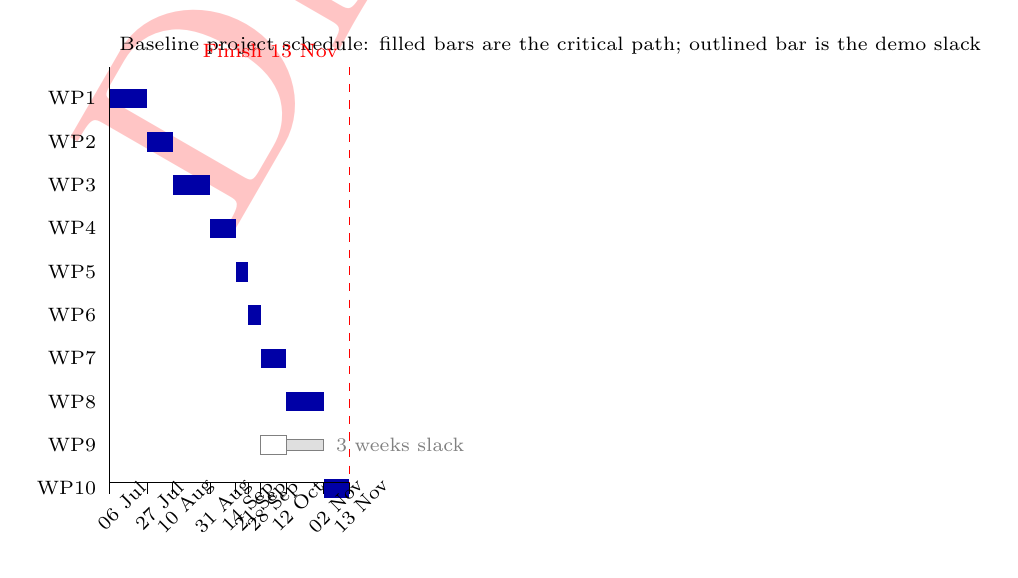
\begin{tikzpicture}[x=0.16cm,y=-0.55cm,font=\scriptsize]
\node[anchor=west] at (0,-1) {Baseline project schedule: filled bars are the critical path; outlined bar is the demo slack};
\foreach \rw/\lb/\st/\en in {0/WP1/0/3,1/WP2/3/5,2/WP3/5/8,3/WP4/8/10,4/WP5/10/11,5/WP6/11/12,6/WP7/12/14,7/WP8/14/17,9/WP10/17/19}{
	\fill[blue!65!black] (\st,\rw) rectangle (\en,\rw+0.45);
	\node[anchor=east] at (-0.3,\rw+0.22) {\lb};
}
\node[anchor=east] at (-0.3,8.22) {WP9};
\draw[gray,fill=white] (12,8) rectangle (14,8.45);
\draw[gray,fill=gray!25] (14,8.1) rectangle (17,8.35);
\node[anchor=west,gray] at (17.2,8.22) {3 weeks slack};
\draw (0,-0.5) -- (0,9.1);
\draw (0,9.1) -- (19,9.1);
\foreach \x/\m in {0/06 Jul,3/27 Jul,5/10 Aug,8/31 Aug,10/14 Sep,11/21 Sep,12/28 Sep,14/12 Oct,17/02 Nov,19/13 Nov}{
	\draw (\x,9.1) -- (\x,9.35);
	\node[anchor=north,rotate=45] at (\x,9.35) {\m};
}
\draw[red,dashed] (19,-0.5) -- (19,9.1);
\node[red,anchor=south east] at (18.9,-0.5) {Finish 13 Nov};
\end{tikzpicture}
\end{center}
\tcap{Figure 1 -- Baseline-vs-actual schedule. Critical path: WP1 $\rightarrow$ WP2 $\rightarrow$ WP3 $\rightarrow$ WP4 $\rightarrow$ WP5 $\rightarrow$ WP6 $\rightarrow$ WP7 $\rightarrow$ WP8 $\rightarrow$ WP10. WP3 required 41 GPU hours; WP9 runs in parallel.}

\section{Determining Cost and Budget}
All costs are notional effort values in Indian Rupees. Student effort is valued at Rs. 1,600 per person-day (Rs. 200 per hour for 8 hours); guide or expert effort is valued at Rs. 1,000 per hour. The workstation, electricity, open-source software and data were already available, so cash expenditure was Rs. 0.

\subsection{Estimate Activity Costs and Total Budgeted Cost}
\begin{longtable}{|L{.28\linewidth}|r|r|r|}
\hline
\hrow\hc{Work package}&\hc{Student effort (Rs.)}&\hc{Guide / other (Rs.)}&\hc{TBC (Rs.)}\\
\hline\endhead
WP1 Literature and problem definition & 36,800 & 2,000 & 38,800\\\hline
WP2 Asset collection & 24,000 & 2,000 & 26,000\\\hline
WP3 SAM leaf extraction & 28,800 & 2,000 & 30,800\\\hline
WP4 Compositor and labelling & 19,200 & 2,000 & 21,200\\\hline
WP5 Dataset packaging & 12,800 & 0 & 12,800\\\hline
WP6 Detector training & 12,800 & 0 & 12,800\\\hline
WP7 Evaluation and analysis & 19,200 & 2,000 & 21,200\\\hline
WP8 Real-UAV transfer study & 28,800 & 2,000 & 30,800\\\hline
WP9 Demo application & 12,800 & 0 & 12,800\\\hline
WP10 Paper and report & 24,000 & 2,000 & 26,000\\\hline
\textbf{Total budgeted cost} & \textbf{219,200} & \textbf{14,000} & \textbf{233,200}\\\hline
\textbf{Contingency reserve (10\%)} & & & \textbf{23,320}\\\hline
\textbf{Funding limit} & & & \textbf{256,520}\\\hline
\end{longtable}
The estimate is a planning baseline for Review 2 and is separate from the earlier technical-paper effort log. It makes the resources behind the ten work packages explicit without inventing cash purchases.

\subsection{Time-Phased Budget and Earned Value}
\begin{longtable}{|L{.27\linewidth}|r|r|r|r|r|}
\hline
\hrow\hc{Period}&\hc{Jul}&\hc{Aug}&\hc{Sep}&\hc{Oct--Nov}&\hc{Cumulative (Rs.)}\\
\hline\endhead
Planned value (PV) & 38,800 & 56,800 & 62,600 & 75,000 & 233,200\\\hline
Earned value (EV) & 38,800 & 56,800 & 62,600 & 75,000 & 233,200\\\hline
Actual cost (AC) & 38,800 & 58,400 & 65,800 & 78,200 & 241,200\\\hline
\end{longtable}
At closure, all ten work packages are complete, so EV equals the total budgeted cost. CPI is $EV/AC=233,200/241,200=0.967$ and cost variance is $EV-AC=-Rs.\,8,000$. Schedule variance is zero because all critical-path deliverables were completed within the baseline window. The actual cost remains within the Rs. 23,320 reserve, leaving Rs. 15,320.

\subsection{Cost Forecast at Completion}
At closure, the most reliable estimate at completion is the actual cost, Rs. 241,200. A CPI-based forecast gives $BAC/CPI=233,200/0.967\approx Rs.\,241,200$, which agrees with the observed cost. The funding-limit TCPI is not constraining because the reserve covers the Rs. 8,000 overrun.

\subsection{Tools, Technology Stack and Code Quality}
\begin{longtable}{|L{.38\linewidth}|L{.48\linewidth}|}
\hline
\hrow\hc{Tool / version}&\hc{Why}\\
\hline\endhead
Python 3.13, PyTorch 2.11, CUDA 12.8 & GPU training on RTX A5000 (24 GB)\\\hline
Ultralytics 8.4.154 & One API for YOLO11 and RT-DETR\\\hline
Segment Anything (ViT-B) & Zero-shot masks without labels\\\hline
Pillow, NumPy, OpenCV & CPU compositing and HSV tiling\\\hline
onnxruntime-web 1.20.1 & Offline in-browser inference\\\hline
Git and Git LFS & Versioned weights and runs\\\hline
\end{longtable}
Pipeline modules are \texttt{segment\_leaf.py}, \texttt{backgrounds.py}, \texttt{generate\_synthetic.py}, \texttt{prepare\_yolo\_dataset.py}, \texttt{train\_{yolo11m,rtdetr}.py}, \texttt{test\_models.py}, \texttt{run\_cv\_experiments.py} and the \texttt{implementation-app/} PWA. Each stage reads the previous stage's folder; parameters live in the scripts. Dataset downloads, launching stages and ONNX export remain manual. The demo runs with \texttt{python implementation-app/tools/serve.py 8080}.

The repository contains one script per stage, requirements, data configuration and a demo README. Reproducibility uses fixed seeds (split 42, training 0); demo numbers are recomputed from \texttt{runs/}. Testing included a held-out split, checkpoint re-evaluation and a throughput test of 67.7 FPS (14.8 ms per tile). No automated unit-test suite exists yet.

\subsection{Training Configuration and Reproducibility}
Both detectors started from COCO weights at 640 px, used AdamW for 40 epochs, linear learning-rate decay to 1\%, weight decay $5\times10^{-4}$, three warm-up epochs, AMP, seed 0, and mosaic disabled for the last 10 epochs. YOLOv11m used batch 16 and learning rate $10^{-3}$; RT-DETR-L used batch 8 and $10^{-4}$. Training took 9.3 and 37.2 minutes respectively. Early stopping with patience 15 did not trigger.

The implementation chain is \texttt{segment\_leaf} $\rightarrow$ \texttt{backgrounds} $\rightarrow$ \texttt{generate\_synthetic} $\rightarrow$ \texttt{prepare\_yolo\_dataset} $\rightarrow$ \texttt{train} $\rightarrow$ \texttt{test\_models} $\rightarrow$ \texttt{prepare\_real\_cv} $\rightarrow$ \texttt{run\_cv\_experiments} $\rightarrow$ web app. Stages communicate through RGBA PNG cutouts, JPEG tile folders, YOLO text labels, \texttt{data.yaml}, fold lists and a JSON result cache.

\section{Managing Risk}
\subsection{Defects Found and Resolved}
\begin{itemize}[leftmargin=*]
\item One SAM file-write failure was reprocessed, producing 18,163 cutouts.
\item A random patch split leaked near-duplicates and produced 0.88 mAP@50; it was replaced with leave-one-plot-out CV.
\item A CUDA illegal-memory crash from two jobs on one GPU was resolved by serial execution; CV resumes from cache.
\item A paper-versus-disk audit found that label files lacked a trailing newline, so \texttt{wc -l} undercounted one box per image (56,571 versus 57,771). The count was corrected by parsing.
\end{itemize}

\subsection{Risk Register}
\begin{longtable}{|L{.31\linewidth}|c|c|L{.39\linewidth}|L{.17\linewidth}|}
\hline
\hrow\hc{Risk}&\hc{L}&\hc{I}&\hc{Mitigation}&\hc{Trigger}\\
\hline\endhead
Sim-to-real gap & H & H & Real-UAV CV and fine-tuning & AUC approximately 0.5\\\hline
GPU job crash & M & M & One job per GPU and resumable cache & CUDA error\\\hline
Data leakage & M & H & Plot-level splits & Too-good scores\\\hline
Paper over page limit & H & M & Cut text and figures & More than 6 pages\\\hline
Numbers drift from code & M & H & Audit; compute, never type & Count mismatch\\\hline
\end{longtable}
The GPU crash on 30 Oct stopped multi-seed CV after 4 of 16 runs. It was diagnosed as GPU contention, rerun alone from cache and completed the same day. Zero-shot transfer reached chance level and redirected effort to fine-tuning.

\subsection{Risk Response Plan}
\begin{longtable}{|L{.25\linewidth}|L{.18\linewidth}|L{.34\linewidth}|L{.14\linewidth}|}
\hline
\hrow\hc{Risk}&\hc{Response}&\hc{Action}&\hc{Owner}\\
\hline\endhead
Sim-to-real gap & Mitigate & Use plot-level CV, document the scale and NIR gap, and prioritise camera-matched synthesis. & Shakthi\\\hline
GPU crash & Mitigate & Run one job at a time, cache fold outputs and resume from the last completed run. & Vedantha\\\hline
Data leakage & Avoid & Split by whole plot for real data and retain asset-sharing as an explicit synthetic limitation. & Hemanth\\\hline
Page-limit risk & Mitigate & Track paper length during weekly review and move technical evidence to appendices. & Hemanth\\\hline
Number drift & Avoid & Recompute figures from stored runs and parse labels rather than trusting line counts. & All members\\\hline
Mask quality uncertainty & Accept and monitor & Record that manual-mask IoU and a GrabCut baseline were not measured; add mask audit to future work. & Shakthi\\\hline
\end{longtable}

\subsection{Risk Monitoring Record}
The sim-to-real risk occurred immediately in the zero-shot study, producing AUC 0.48. The response was to use the public real-UAV data for plot-level fine-tuning and to report the negative low-data result. The GPU risk occurred during the multi-seed run; serial execution and cache recovery completed it on 30 Oct. The leakage risk was detected when a random split produced 0.88 mAP@50; the split was rejected and replaced by leave-one-plot-out evaluation. The number-drift risk occurred in the label count and speed figures; both were corrected through an audit before the report was finalised.

\section{The Project Team}
\subsection{Team Effectiveness}
\begin{longtable}{|L{.34\linewidth}|c|L{.44\linewidth}|}
\hline
\hrow\hc{Characteristic}&\hc{Rating}&\hc{Evidence}\\
\hline\endhead
Clear objective & 5 & Shared metric targets: labels, mAP, AUC, FPS and reproducibility.\\\hline
Clear roles & 4 & One primary owner per work package and shared support during integration.\\\hline
Results orientation & 5 & The team rejected the leaky split and reported the zero-shot failure rather than hiding it.\\\hline
Collaboration & 4 & SAM, compositor, detector and transfer stages were reviewed across members.\\\hline
Trust and transparency & 4 & GPU failures, count corrections and missing ablations were recorded openly.\\\hline
\end{longtable}

\subsection{Conflict and Problem Solving}
The central scope decision was whether to present the synthetic detector as a field-ready result or to treat transfer failure as a research finding. The team used a collaborating approach: compare the random split with plot-level CV, inspect the scale and colour gap, rerun the real data with three seeds, and revise the claim. The chosen solution was to report strong synthetic performance, chance-level zero-shot transfer, and a conditional full-data gain without claiming deployment readiness.

\begin{longtable}{|c|L{.70\linewidth}|}
\hline
\hrow\hc{Step}&\hc{Evidence-based action}\\
\hline\endhead
1 & Define the problem: synthetic metrics may be inflated and transfer may fail.\\\hline
2 & Identify causes: shared assets, eight-fold scale gap, NIR-shifted colour, weak patch labels and undertrained RT-DETR.\\\hline
3 & Test alternatives: random split versus plot-level CV, zero-shot versus real-only versus synthetic pretraining.\\\hline
4 & Set decision criteria: no leakage, reproducible numbers, honest caveats and finish within the review window.\\\hline
5 & Select the response: leave-one-plot-out CV, three-seed full-data comparison and camera-matched synthesis as future work.\\\hline
6 & Verify outcome: AUC 0.59 to 0.68 with full real data, 8 of 12 paired wins, no low-data gain.\\\hline
\end{longtable}
\subsection{Experimental Setup and Evaluation Metrics}
The synthetic dataset contains 1,200 composites, 6 classes balanced by instance (9.5--9.8k each), and a 960/120/120 split with seed 42. The real UAV dataset [8] contains 3,157 patches at 256 px and 0.3 mm/px, across 5 plots, with 1,027 infected and 2,130 healthy patches under leave-one-plot-out evaluation.

\begin{longtable}{|L{.28\linewidth}|L{.27\linewidth}|L{.27\linewidth}|}
\hline
\hrow\hc{Setting}&\hc{YOLOv11m}&\hc{RT-DETR-L}\\
\hline\endhead
Batch / learning rate & 16 / $10^{-3}$ & 8 / $10^{-4}$\\\hline
Optimiser, epochs & AdamW, 40 & AdamW, 40\\\hline
Input, initialisation & 640, COCO & 640, COCO\\\hline
\end{longtable}

mAP@50 and mAP@50--95 measure detection quality; 50--95 rewards tight boxes. Precision, recall and F1 use the F1-optimal threshold. FPS at batch 1 and FP32 measures survey-time feasibility. AUC and AP are used for real data because only patch labels exist. Baselines were RT-DETR-L on the same data and budget, real-only YOLOv11m with COCO initialisation, and a zero-shot synthetic model.

For real-patch evaluation, each infected patch receives a weak box covering its central 70\%. The patch score is the highest confidence of any disease detection, and AUC, AP and validation-selected F1 are reported. Labelling every patch as infected already gives F1 approximately 0.65, so F1 alone is not sufficient. Leave-one-plot-out is used because patches from one image and plot are near-duplicates.

\subsection{Comparative Benchmarking}
\begin{longtable}{|L{.28\linewidth}|r|r|r|r|r|r|}
\hline
\hrow\hc{Model}&\hc{Params}&\hc{P}&\hc{R}&\hc{F1}&\hc{mAP@50}&\hc{mAP@50--95}\\
\hline\endhead
YOLOv11m (CNN) & 20.1 M & 0.918 & 0.836 & 0.875 & 0.907 & 0.733\\\hline
RT-DETR-L (Transformer) & 32.8 M & 0.801 & 0.704 & 0.749 & 0.761 & 0.542\\\hline
\end{longtable}
YOLOv11m wins by +0.146 mAP@50, +0.191 mAP@50--95 and 2.2 times the speed. RT-DETR-L was undertrained: it was below 0.31 mAP@50 for 26 of 40 epochs and still rising at 40.

The re-measured inference speed is median batch-one FP32 performance over five rounds after 30 warm-up images on the RTX A5000: YOLOv11m 67.7 FPS (14.8 ms) and RT-DETR-L 31.2 FPS (32.0 ms). Earlier unreproducible values of 74.7 and 33.6 FPS are not used.

\section{Lessons Learned and Conclusion}
\subsection{Results on the Held-Out Synthetic Test Split}
\begin{longtable}{|L{.34\linewidth}|r|r|}
\hline
\hrow\hc{Class}&\hc{mAP@50}&\hc{mAP@50--95}\\
\hline\endhead
Potato Early Blight & 0.950 & 0.801\\\hline
Potato Late Blight & 0.912 & 0.758\\\hline
Potato Healthy & 0.955 & 0.824\\\hline
Tomato Early Blight & 0.895 & 0.688\\\hline
Tomato Late Blight & 0.801 & 0.584\\\hline
Tomato Healthy & 0.927 & 0.742\\\hline
Mean (YOLOv11m) & 0.907 & 0.733\\\hline
\end{longtable}
The worst class was Tomato Late Blight, with recall 0.679 and 16\% missed as background. The validation--test gap was 0.009--0.016. This is a single seed and the test shares assets with training.

\subsection{Validation on Real UAV Imagery}
\begin{longtable}{|L{.27\linewidth}|r|r|r|}
\hline
\hrow\hc{Real data}&\hc{Real-only}&\hc{Synthetic to real}&\hc{Gain}\\
\hline\endhead
0\% (zero-shot) & -- & 0.48 $\pm$ 0.01 & --\\\hline
10\% & 0.47 $\pm$ 0.05 & 0.52 $\pm$ 0.04 & +0.05\\\hline
25\% & 0.56 $\pm$ 0.04 & 0.56 $\pm$ 0.01 & 0.00\\\hline
100\% (3 seeds) & 0.59 $\pm$ 0.04 & 0.68 $\pm$ 0.13 & +0.09\\\hline
\end{longtable}
Zero-shot fails at chance-level AUC because real patches are eight times finer, contain lesions rather than leaves, and are NIR-shifted. Pretraining helps with full data but unevenly: mean per-plot gains were +0.02, --0.03, +0.25 and +0.11, winning 8 of 12 paired runs. There was no gain at 10--25\%. The 100\% rows are four folds by three seeds; the single-seed gain of +0.13 shrank to +0.09.

\subsection{Novelty and Research Contribution}
AgroEye turns real photographed PlantVillage disease leaves into UAV-scale, rotation-aware labelled scenes and tests them honestly on real UAV imagery under a leakage-free split. Its new contributions are a mask score that credits diseased hues, real photographed lesions instead of generated targets, seven-factor UAV-scale composition with canopy-density clusters, labels from rotated alpha, plot-level CV and an in-browser demo.

\subsection{Optimization and Ablation Study}
Native-resolution tiling keeps soil texture; an IoU guard of 0.50 permits partial canopy overlap without duplicate boxes; RT-DETR-L uses batch 8 and learning rate $10^{-4}$; mosaic is disabled for the last 10 epochs and AMP training is used. The per-factor ablation has not been run. Planned runs are naive copy-paste, without feathering, without shadow, without GSD scaling and without sensor blur. Unsuccessful approaches were zero-shot transfer (AUC 0.48), any-blight scoring (0.50), the random patch split and RT-DETR-L at a 40-epoch budget.

\subsection{Conclusion and Future Work}
O1--O3 achieved an annotation-free pipeline from PlantVillage to labelled UAV-style scenes, with trained and compared detectors. O4 was partially achieved through the first leakage-free real-UAV transfer test. O5 achieved a working in-browser demo. Future work is camera-matched synthesis at target GSD with hue and channel jitter, factor ablation, asset-disjoint splits, real box labels on several hundred UAV frames and a PlantDoc [13] test, fair RT-DETR training to convergence with at least three seeds, and single-crop scenes with clustered infection.

\section{Individual Contribution and Reflection}
\subsection{Project Report and Documentation Status}
The complete draft in the BMSCE template has 79 pages, 6 chapters and 3 appendices: Introduction, Literature Review, Methodology, Implementation, Results and Discussion, and Conclusion. It has 22 figures, 21 tables and 41 references; metrics were re-checked against \texttt{runs/} and \texttt{results/}. Formatting uses IEEE citation style with numbered figures and tables. Appendices contain source-code excerpts, dataset configuration, training and reproduction commands, and all 48 runs of the real-UAV study.

\subsection{SDG Mapping and Societal Impact}
\begin{longtable}{|L{.18\linewidth}|L{.65\linewidth}|}
\hline
\hrow\hc{Target}&\hc{Link to AgroEye}\\
\hline\endhead
SDG 2.4 & Early disease detection supports resilient, sustainable food production\\\hline
SDG 2.3 & Low-cost scouting for small-scale producers\\\hline
SDG 12.3 & Reduce crop losses at the production stage\\\hline
SDG 9.5 & Open, reproducible agricultural AI research capacity\\\hline
\end{longtable}
Stakeholders are smallholder farmers, agronomists, extension officers and drone service providers. Results show 57,771 labelled boxes with zero manual annotation, 14.8 ms per 640 px tile, and synthetic pretraining lifting full-data real AUC from 0.59 to 0.68. Yield-loss and fungicide reductions were not measured; real-field use remains limited to one disease, one season and patch labels.

\subsection{Research Paper Status}
The paper \textit{AgroEye: A SAM-Based Synthetic Data Pipeline for UAV-Style Crop Disease Detection, with a Transfer Study on Real UAV Imagery} is drafted and internally reviewed for IEEE CSITSS, hosted by RVCE, in IEEEtran format. The current build is 10 pages and its open item is checking the venue limit. Counts, FPS and three-seed real-UAV results were corrected on 30 Oct 2026. Funding is from the BMSCE Faculty Research Promotion Scheme, R\&D/FRPS-3/2025-26/CS/1-20. Similarity-score evidence and submission acknowledgement remain to be attached when available.

\section*{Consistency Checks}
\addcontentsline{toc}{section}{Consistency Checks}
\begin{longtable}{|L{.38\linewidth}|L{.44\linewidth}|L{.10\linewidth}|}
\hline
\hrow\hc{Check}&\hc{Evidence}&\hc{Status}\\
\hline\endhead
Synthetic assets are counted from the dataset audit & 18,163 SAM cutouts; 6,652 used; 1,200 composites; 57,771 boxes & Yes\\\hline
Synthetic test performance is reported from the held-out split & YOLOv11m mAP@50 0.907; mAP@50--95 0.733 & Yes\\\hline
Real transfer results use leakage-free evaluation & Leave-one-plot-out; full-data AUC 0.59 to 0.68 & Yes\\\hline
The throughput claim is reproducible & 67.7 FPS and 14.8 ms per tile & Yes\\\hline
The box count was corrected by parsing files & 57,771 rather than the newline-based 56,571 count & Yes\\\hline
\end{longtable}

\newpage
\section*{Appendices}
\addcontentsline{toc}{section}{Appendices}
\subsection*{Appendix A: Dataset and Evaluation Audit}
\addcontentsline{toc}{subsection}{Appendix A: Dataset and Evaluation Audit}
The synthetic test split is independent in arrangement but not asset-disjoint: the 176 aerial tiles and 6,652 selected cutouts are reused across splits. Each cutout appears approximately eight times overall, and the Potato Healthy pool is reused approximately 60 times. Therefore the 0.907 mAP@50 result is an upper bound for generalisation within the synthetic distribution, not evidence of transfer to unseen fields.

The real dataset is the 2022 subset of Wieme et al. [8]: potato early blight caused by \textit{A. solani}, acquired at 10 m with a 42 MP camera, 135 mm lens and the NIR-blocking filter removed. It contains 3,157 patches of 256 px from 281 drone images, 5 plots and 4 dates, with 1,027 infected and 2,130 healthy patches. Plot 5 is 96\% healthy and the resolution is 0.3 mm/px, approximately eight times finer than the synthetic imagery.

Leave-one-plot-out evaluation prevents near-duplicate patches from the same image or field entering both training and test. Each fold tests one whole plot, validates on the next and trains on the remaining plots plus plot 5. The discarded random patch split produced 0.88 mAP@50 and was judged leaky.

\begin{longtable}{|L{.34\linewidth}|L{.49\linewidth}|}
\hline
\hrow\hc{Validation check}&\hc{Result}\\
\hline\endhead
Cutouts & 18,163 non-empty single-component outputs\\\hline
Labels & 57,771 parsed label lines; 0 invalid labels\\\hline
Split integrity & No image appears in two synthetic splits\\\hline
Fold integrity & No plot appears in two parts of a real-UAV fold\\\hline
Training reproduction & Checkpoint re-evaluation reproduces reported metrics\\\hline
Mask limitation & Manual-mask IoU and GrabCut/Otsu comparison were not measured\\\hline
\end{longtable}

\subsection*{Appendix B: Review Questions and Evidence}
\addcontentsline{toc}{subsection}{Appendix B: Review Questions and Evidence}
\textbf{Why not annotate real drone images?} A 640 px tile can contain more than 50 small leaves, each requiring a tight box and expert disease label. The available in-house flights were not annotated, and the public UAV dataset has patch labels only.

\textbf{Why include yellow and brown in the mask score?} A green threshold would remove diseased tissue. The colour term therefore scores green and yellow--brown HSV regions. The weights were set by hand, not tuned, and SAM mask IoU was not measured.

\textbf{Why native-resolution tiles?} Downscaling large aerial images erases furrows and clods and changes the scale relationship between leaves and backgrounds. The 65 sources were converted into 176 tiles and grouped by HSV green ratio.

\textbf{Why did the annotation count change?} Label files lacked a trailing newline. Line counting merged the last line of one file with the first line of the next, undercounting one box per image. Parsing every file corrected the count to 57,771.

\textbf{Why does zero-shot transfer fail?} The real patches are approximately eight times finer, show lesions rather than whole leaves, and have NIR-shifted colour. The synthetic model had not seen that scale or camera response.

\textbf{Is the real-data gain statistically significant?} No significance claim is made. The full-data mean gain is $+0.09\pm0.13$ over three seeds; plot gains are $+0.02$, $-0.03$, $+0.25$ and $+0.11$, with 8 of 12 paired wins.

\textbf{Did the project reduce the required real-data volume?} No. At 10\% and 25\% real data, both initialisations remain near chance and differ by at most 0.05 AUC.

\textbf{Did the project run an ablation of the seven factors?} No. The planned ablation compares naive copy-paste with one-factor-removed variants on the same test data. No unverified ablation number is reported.

\textbf{What is the next priority?} Camera-matched synthesis at target resolution with hue and channel jitter, followed by factor ablation, asset-disjoint splits, real box labels and a PlantDoc test, converged multi-seed RT-DETR training, clustered single-crop scenes and mask quality control.

\subsection*{Appendix C: Paper and Review Readiness}
\addcontentsline{toc}{subsection}{Appendix C: Paper and Review Readiness}
The review deck has 21 content slides plus a title and questions slide. The report draft has 6 chapters, 3 appendices, 79 pages, 22 figures, 21 tables and 41 references in the BMSCE template. The paper is a 10-page IEEEtran draft for CSITSS, internally reviewed and revised on 29--30 Oct 2026. Before submission, the venue page limit, similarity report and submission acknowledgement must be attached.

The similarity target is at most 20\%, with references excluded; the score, tool and date are not yet recorded in the supplied materials. The project does not claim field deployment, measured yield reduction, measured fungicide reduction, a statistically significant real-UAV gain, perfect SAM masks or a fair-to-convergence Transformer comparison.

\section*{References}
\addcontentsline{toc}{section}{References}
\begin{enumerate}[label={[\arabic*]}]
\item D. P. Hughes and M. Salathé, ``An open access repository of images on plant health to enable the development of mobile disease diagnostics,'' arXiv:1511.08060, 2015.
\item S. P. Mohanty, D. P. Hughes, and M. Salathé, ``Using deep learning for image-based plant disease detection,'' \textit{Front. Plant Sci.}, vol. 7, 1419, 2016.
\item D. Dwibedi, I. Misra, and M. Hebert, ``Cut, paste and learn: Surprisingly easy synthesis for instance detection,'' in Proc. ICCV, 2017, pp. 1301--1310.
\item J. Tobin et al., ``Domain randomization for transferring deep neural networks from simulation to the real world,'' in Proc. IROS, 2017, pp. 23--30.
\item J. Tremblay et al., ``Training deep networks with synthetic data: Bridging the reality gap by domain randomization,'' in Proc. CVPRW, 2018, pp. 969--977.
\item N. Giakoumoglou, E. M. Pechlivani, and D. Tzovaras, ``Generate-Paste-Blend-Detect: Synthetic dataset for object detection in the agriculture domain,'' \textit{Smart Agric. Technol.}, vol. 5, 100258, 2023.
\item A. Prasad, N. Mehta, M. Horak, and W. D. Bae, ``A two-step machine learning approach for crop disease detection: An application of GAN and UAV technology,'' arXiv:2109.11066, 2021.
\item J. Wieme et al., ``Ultra-high-resolution UAV-imaging and supervised deep learning for accurate detection of Alternaria solani in potato fields,'' \textit{Front. Plant Sci.}, vol. 15, 2024.
\item D. Williams, F. Macfarlane, and A. Britten, ``Leaf Only SAM: A Segment Anything pipeline for zero-shot automated leaf segmentation,'' arXiv:2305.09418, 2023.
\item A. Kirillov et al., ``Segment Anything,'' in Proc. ICCV, 2023, pp. 4015--4026.
\item G. Jocher and J. Qiu, ``Ultralytics YOLO11,'' v11.0.0. [Online]. Available: \url{https://github.com/ultralytics/ultralytics}
\item Y. Zhao et al., ``DETRs beat YOLOs on real-time object detection,'' in Proc. CVPR, 2024, pp. 16965--16974.
\item D. Singh et al., ``PlantDoc: A dataset for visual plant disease detection,'' in Proc. CoDS-COMAD, 2020, pp. 249--253.
\end{enumerate}
\end{document}
